
\begin{figure}[h]
\centering
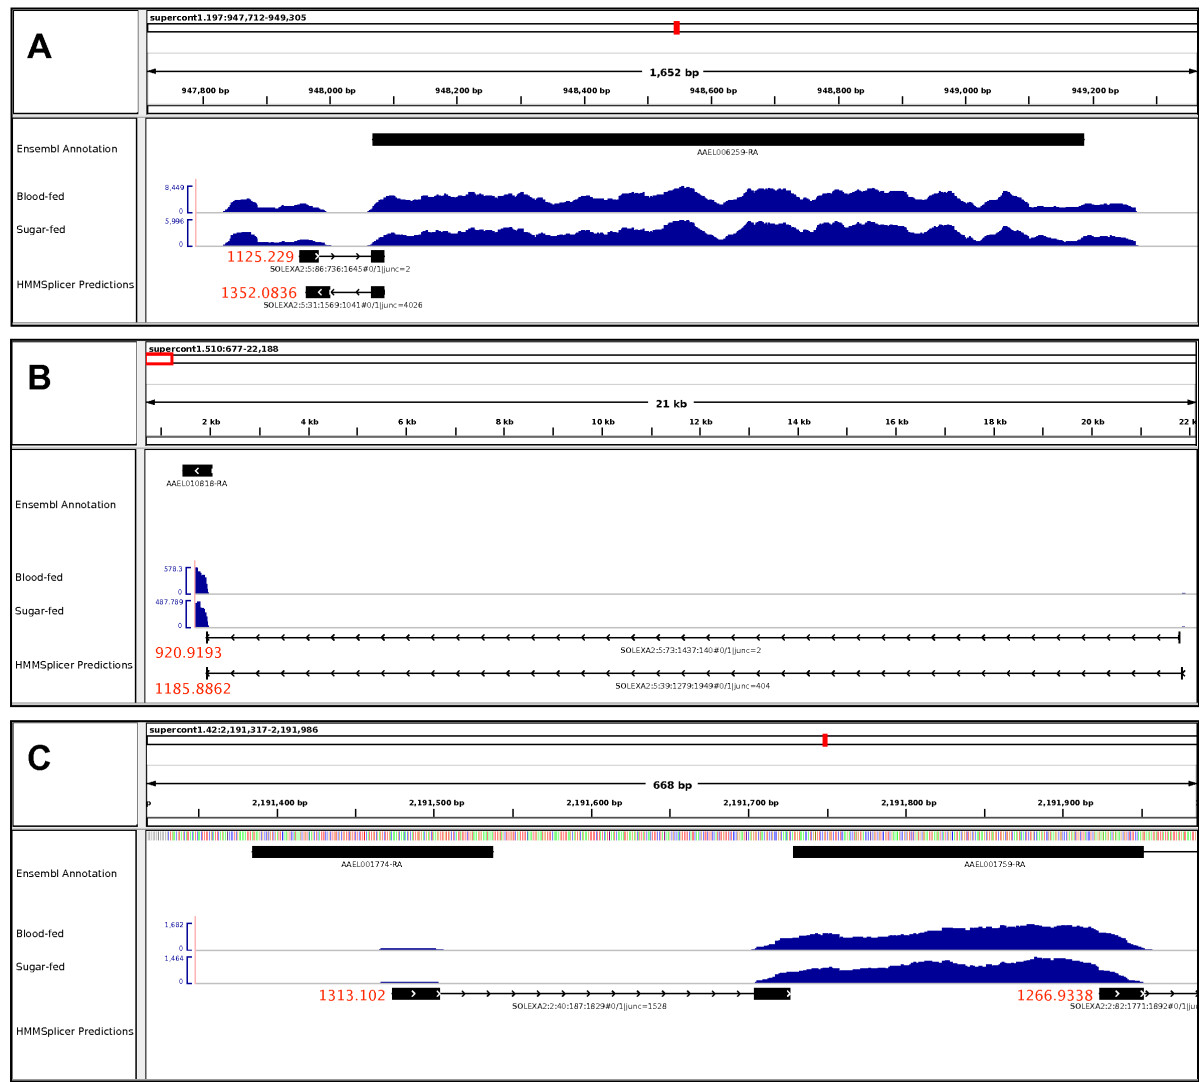
\includegraphics[width=.95\textwidth]{figures/figs/aedesHMMsplice.jpg}

\caption[Examples of amendments to the \Aa\ annotation supported by HMMSplicer results]{\sf \textbf{Examples of amendments to the \Aa\ annotation supported by HMMSplicer results:} Black bars in the top tracks represent the current gene annotations. Blue histograms in the second track represent the non-normalized coverage of RNA-seq reads at each position. The range of the histogram values shown in each view is depicted on the labeled y-axis of each RNA-seq track. Black boxes in the lower track represent splice-site predictions based on the RNA-seq reads using HMMSplicer determined in this study. Each function has a unique identifier listed below and its HMMSplicer score is listed in red. If multiple reads support a single junction, "junc = x" lists the number of supporting reads. This information provides evidence to link two islands of transcription as a single transcription event, therefore, exons of a common mRNA. All predicted junctions shown here also are supported by EST alignments. Genes are (A) AAEL006259; (B) AAEL010818; and (C) AAEL001774 and AAEL001759.

Excerpted from \cite{Bonizzoni2011}}
\label{fig:aedesHMMsplice}
\end{figure}